% Interim report: computationally efficient STAP/GMTI with a 77 GHz FMCW radar
% Build: python report/make_figures.py, then run pdflatex interim_report.tex twice from report/
% (references are inline in thebibliography, so no BibTeX run is needed). Works as-is on Overleaf
% if report/figures/ is uploaded alongside this file.
\documentclass[conference]{IEEEtran}
\usepackage{amsmath,amssymb}
\usepackage{graphicx}
\usepackage{booktabs}
\usepackage{multirow}
\usepackage{cite}
\usepackage{tikz}
\usetikzlibrary{arrows.meta,positioning}
\graphicspath{{figures/}}
\newcommand{\vect}[1]{\mathbf{#1}}
\newcommand{\Hm}{^{\mathsf H}}

\begin{document}

\title{Computationally Efficient Space-Time Adaptive Processing for Ground-Moving-Target Indication with a Low-Cost 77\,GHz FMCW Radar: Interim Report}

\author{\IEEEauthorblockN{Ozair Khan}
\IEEEauthorblockA{\textit{[Affiliation / programme]}\\
\textit{[Supervisor]}}}

\maketitle

\begin{abstract}
This interim report describes progress on a research project that studies space-time adaptive
processing (STAP) for ground-moving-target indication (GMTI) using a commercial TI IWR1843BOOST
77\,GHz FMCW radar with a DCA1000EVM raw-ADC capture card. A complete, tested processing chain
has been built: a physics-based multichannel FMCW simulator, a verified DCA1000 decoder, range,
Doppler, angle and CFAR processing, per-channel calibration, and five STAP filters (non-adaptive,
full-rank MVDR, extended factored (EFA), principal components (PC) and DPCA) with multi-frame
training, forward-backward averaging and power censoring. Three indoor bench captures were decoded
without errors and processed end to end. On the default simulated airborne scenario, MVDR, PC and
EFA reach 23.0, 22.8 and 21.3\,dB output SINR against a 24.1\,dB optimum. Two outdoor experiments
have been designed: a static highway overlook to validate the real-data chain, and a side-looking
vehicle-mounted experiment at 50--100\,km/h for true STAP. Measured run times show that full-rank
STAP at the overlook dimension ($D=512$) costs about 2\,s per range bin on a 4-core CPU. This
motivates the remaining research, which focuses on reducing STAP computation without losing
detection performance, and the report sets out candidate algorithmic and machine-learning
directions and an evaluation plan.
\end{abstract}

\begin{IEEEkeywords}
STAP, GMTI, FMCW radar, MVDR, reduced-dimension STAP, mmWave, DCA1000, clutter suppression
\end{IEEEkeywords}

% ======================================================================
\section{Introduction}
A radar on a moving platform sees stationary ground clutter at a radial velocity that depends on
the look angle, $v_r=-v_p\sin\theta$ for a side-looking array. Clutter therefore lies on a ridge in
angle-Doppler space, and a slow ground mover can share its Doppler with clutter arriving from
another angle. Separating the two needs joint spatial and temporal (space-time) filtering, which
is what STAP provides~\cite{brennan1973,ward1994,klemm2006}. The optimum filter needs the inverse of a
$D\times D$ interference covariance, with $D$ = channels $\times$ pulses. Estimating that covariance
needs roughly $2D$ homogeneous training samples~\cite{rmb1974}, and the computational cost grows
as $\mathcal O(D^3)$ per range bin. Both limits are severe for low-cost automotive mmWave radars.
These radars have few channels but many chirps, a short range swath, and modest on-board compute.

\textbf{Objectives.} (i) Build a verified end-to-end STAP/GMTI chain for the IWR1843BOOST +
DCA1000EVM, (ii) collect real static and moving-platform data, (iii) benchmark conventional
full-rank STAP against reduced-dimension filters on identical data, training rules and Doppler
hypotheses, and (iv) investigate algorithmic and learning-based methods that reduce computation
with a quantified detection-performance cost.

% ======================================================================
\section{Progress to Date}
\subsection{Software}
The Python package \texttt{radar\_stap} (NumPy/SciPy, optional CuPy backend) implements the
chain in Fig.~\ref{fig:pipeline}. All sign conventions (mixer, radial velocity, angle, space-time
stacking) are defined once and checked by tests. The test suite has 124 tests (unit, physics,
hardware path, integration). On the current repository copy, 121 pass. The 3 failures come only
from a legacy bench configuration file that is absent from that copy, not from processing code.
A capture is only processed after a stage-gating check passes. Each stage (decode, range,
Doppler, angle, STAP) runs only when the metadata it needs has been verified. The provenance of
every waveform field is recorded.

\begin{figure}[t]
\centering
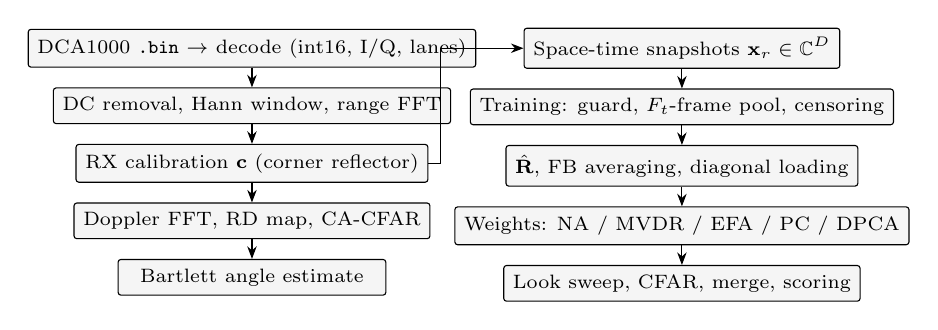
\begin{tikzpicture}[node distance=2.5mm, every node/.style={font=\scriptsize},
  blk/.style={draw, rounded corners=1pt, fill=gray!8, minimum width=34mm, minimum height=4.2mm, align=center},
  arr/.style={-{Stealth[length=1.6mm]}}]
\node[blk] (adc) {DCA1000 \texttt{.bin} $\rightarrow$ decode (int16, I/Q, lanes)};
\node[blk, below=of adc] (rng) {DC removal, Hann window, range FFT};
\node[blk, below=of rng] (cal) {RX calibration $\vect c$ (corner reflector)};
\node[blk, below=of cal] (dop) {Doppler FFT, RD map, CA-CFAR};
\node[blk, below=of dop] (ang) {Bartlett angle estimate};
\node[blk, right=6mm of adc] (snap) {Space-time snapshots $\vect x_r\in\mathbb C^{D}$};
\node[blk, below=of snap] (trn) {Training: guard, $F_t$-frame pool, censoring};
\node[blk, below=of trn] (cov) {$\hat{\vect R}$, FB averaging, diagonal loading};
\node[blk, below=of cov] (w) {Weights: NA / MVDR / EFA / PC / DPCA};
\node[blk, below=of w] (det) {Look sweep, CFAR, merge, scoring};
\draw[arr] (adc)--(rng); \draw[arr] (rng)--(cal); \draw[arr] (cal)--(dop); \draw[arr] (dop)--(ang);
\draw[arr] (cal.east) -- ++(1.5mm,0) |- (snap.west);
\draw[arr] (snap)--(trn); \draw[arr] (trn)--(cov); \draw[arr] (cov)--(w); \draw[arr] (w)--(det);
\end{tikzpicture}
\caption{Processing chain. Left: conventional range-Doppler-angle path. Right: STAP path
operating on calibrated, range-compressed data.}
\label{fig:pipeline}
\end{figure}

\subsection{Simulation results}
The simulator computes the exact bistatic path length per scatterer, receiver and chirp. Range
migration and range-Doppler coupling are therefore included. Clutter is modelled as thousands of
Rayleigh ground scatterers with coherent space-time structure. For the default side-looking
scenario (8\,m/s platform, 4~RX, 16~chirps, $D=64$, 160 training bins), the clairvoyant clutter
eigenspectrum has 13 eigenvalues more than 10\,dB above the noise floor. This matches Brennan's
rule~\cite{ward1994}. Table~\ref{tab:sinr} gives output SINR and Monte-Carlo detection rates.

\begin{table}[t]
\centering
\caption{Default simulated scenario: SINR at a +3\,m/s in-beam mover whose Doppler is shared with
sidelobe clutter (input SINR $-16.4$\,dB, optimum 24.1\,dB). $P_D$: 40 Monte-Carlo trials, design
per-cell $P_{FA}=10^{-3}$, 95\,\% Wilson intervals.}
\label{tab:sinr}
\begin{tabular}{lccc}
\toprule
Method & SINR [dB] & $P_D$ [95\,\% CI] & $P_{FA}$ \\
\midrule
Non-adaptive & 6.4 & 0.00 [0.00, 0.09] & $7.1\times10^{-3}$\\
MVDR ($D=64$) & 23.0 & 0.88 [0.74, 0.95] & $1.7\times10^{-3}$\\
EFA ($r=12$) & 21.3 & 0.57 [0.42, 0.71] & $2.2\times10^{-3}$\\
PC & 22.8 & 0.80 [0.65, 0.90] & $1.7\times10^{-3}$\\
\bottomrule
\end{tabular}
\end{table}

EFA gives up about 2\,dB of SINR compared with MVDR. In return it solves a 12-dimensional
problem that needs about 24 instead of about 128 training bins. Its runtime only becomes lower
than MVDR's at larger $D$, which is the trade-off this project studies.

\subsection{Indoor bench captures (real data)}
Three captures were recorded with the legacy bench waveform (3-TX TDM, 128 loops, 256 samples,
64 frames, 100.7\,MB per capture). All three decoded with 0 dropped bytes and 0 out-of-range ADC values.
The channel RMS was 399--429 ADC codes out of 32767, so the receiver has ample headroom.
Room reflectors were found consistently at 0.71, 1.27, 2.97, 4.35, 4.52 and 6.68\,m
(Fig.~\ref{fig:bench}). Capture~001 contains a walking person at 0.15--1.2\,m/s. Two lessons
shaped the outdoor designs. (i)~With a static radar there is no clutter ridge, so STAP has no
advantage over conventional processing. (ii)~3-TX TDM gives $D=12\times128=1536$ with only 64
training bins, so full-rank STAP is impossible ($K<D$, Fig.~\ref{fig:rmb}). TDM also couples
radial speed into apparent angle. All further experiments therefore use a single TX.

\begin{figure*}[t]
\centering
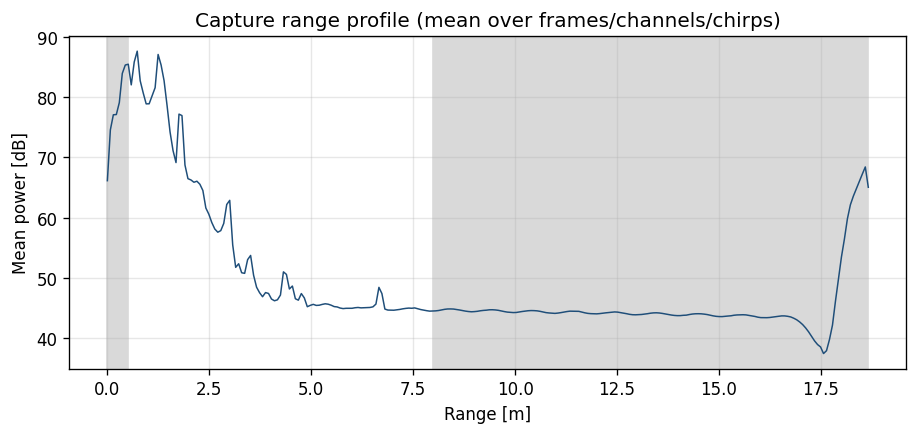
\includegraphics[width=0.48\textwidth]{bench001_range_profile.png}\hfill
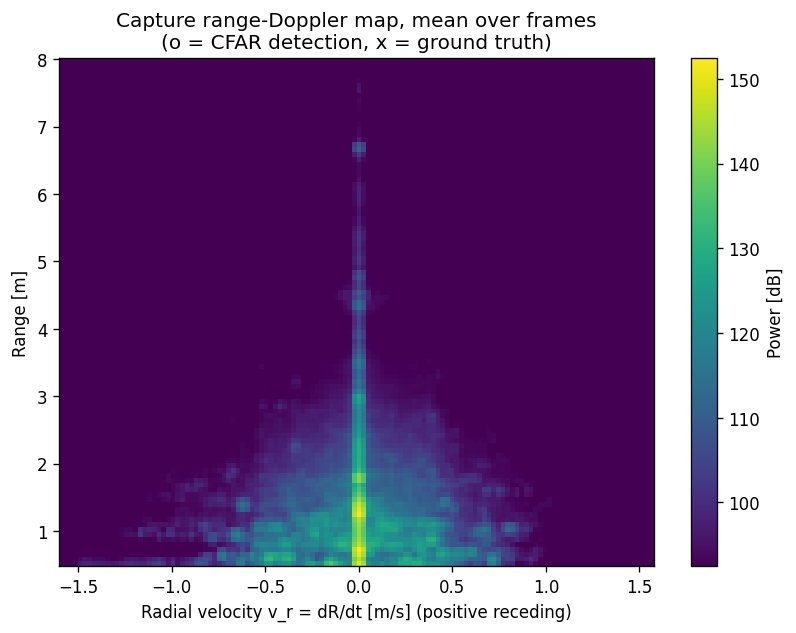
\includegraphics[width=0.48\textwidth]{bench001_range_doppler_mean.png}
\caption{Real bench capture 001 (IWR1843BOOST + DCA1000EVM, indoor): (a) range profile, (b)
range-Doppler map averaged over 64 frames. Static reflectors sit at 0\,m/s. The walking person
appears as off-zero Doppler energy. Bin spacing 0.073\,m, $v_{max}=\pm1.59$\,m/s.}
\label{fig:bench}
\end{figure*}

\subsection{Synthetic end-to-end test through the hardware path}
A synthetic version of Experiment~1 was written to raw DCA1000 files and processed exactly like
real data. It covers 12 lanes of traffic, ground clutter, barrier posts, a gantry and poles,
injected per-RX phase errors of $[0,25,-15,40]^\circ$, and 16-bit quantisation. The test
recovers the calibration to within $0.61^\circ$ of the injected phases. A check reflector at
$27^\circ$ is measured at $26.90^\circ$ with calibration and $24.20^\circ$ without. In the
conventional chain (17 vehicles, 12 frames), calibration reduces the vehicle angle error from
$-3.3^\circ$ mean / $3.7^\circ$ RMS to $0.0^\circ$ / $1.3^\circ$. The overall $P_D$ is 0.18 and is
limited by SNR. Under the assumed link budget most vehicles beyond about 140\,m fall below 13\,dB
integrated SNR. In frame~0, 3 of the 4 vehicles above 13\,dB were detected. The miss was a
near-boresight car ($-6^\circ$, $-3.6$\,m/s, 16\,dB), and its cause has not yet been diagnosed.
These numbers depend on the assumed link budget and should be read as a functional check of the
chain, not as a performance prediction. The full STAP run of this
test could not be completed in the available compute budget (Section~\ref{sec:cost}).

% ======================================================================
\section{Engineering Details}
\subsection{Hardware and data path}
The IWR1843BOOST has 3~TX and 4~RX antennas. The RX elements form a uniform linear array at
$\lambda/2$ spacing, and only TX1 is used. The radar operates at 77\,GHz with complex baseband
sampling at 10\,Msps and 16-bit ADC words. The DCA1000EVM streams the ADC data over 2-lane LVDS
(DDR, 600\,Mbps) and raw-mode Ethernet. The host is 192.168.33.30 and the FPGA is 192.168.33.180
(config port 4096, data port 4098). The binary layout is \texttt{two\_sample\_blocks} (I-first)
and \texttt{rx\_planar\_per\_chirp}, little-endian int16, as verified on the bench captures. The
RX gain is 30\,dB, and the high-pass filter corners are 175/350\,kHz.

\subsection{Waveform design}
Table~\ref{tab:waveform} lists the waveforms. The derived quantities are computed from the YAML
configurations. The wavelength is taken at the centre of the sampled sweep,
$f_c+S(t_{adc}+N/2f_s)$. Both outdoor waveforms share the same 33.5\,$\mu$s chirp period (4\,$\mu$s
idle + 29.5\,$\mu$s ramp). This is the longest period that keeps $v_{max}\approx29$\,m/s
(105\,km/h, Fig.~\ref{fig:waveform}a). The 24\,$\mu$s ADC window is the longest that fits within
that period, and it sets the range resolution (Fig.~\ref{fig:waveform}b). The slopes are rounded
to the TI slope LSB of 48.2797\,kHz/$\mu$s.

\begin{table}[t]
\centering
\caption{Waveforms and derived quantities (TX1 only for outdoor experiments).}
\label{tab:waveform}
\setlength{\tabcolsep}{3pt}
\begin{tabular}{lccc}
\toprule
Quantity & Bench (legacy) & Exp.~1 overlook & Exp.~2 vehicle \\
\midrule
TX schedule & TX1--3 TDM & TX1 & TX1 \\
Slope $S$ [MHz/$\mu$s] & 80 & 4.490 & 11.008 \\
ADC samples $N$ / $f_s$ & 256 / 10\,Msps & 240 / 10\,Msps & 240 / 10\,Msps \\
Chirp period $T_c$ [$\mu$s] & 200 & 33.5 & 33.5 \\
Loops per frame $L$ & 128 & 128 & 16 \\
Sampled bandwidth $B$ [MHz] & 2048 & 107.8 & 264.2 \\
Range resolution $c/2B$ [m] & 0.073 & 1.39 & 0.57 \\
Range-bin spacing [m] & 0.073 & 1.30 & 0.53 \\
IF-limited range $cf_s/2S$ [m] & 18.7 & 334 & 136 \\
Processed range [m] & -- & 40--290 & 4--115 \\
$v_{max}=\lambda/4T_{slow}$ [m/s] & $\pm1.59$ & $\pm29.0$ & $\pm29.0$ \\
Velocity resolution [m/s] & 0.025 & 0.45 & 3.62 \\
CPI $L\,T_{slow}$ [ms] & 76.8 & 4.29 & 0.54 \\
Frame period / frames & -- / 64 & 50\,ms / 600 & 20\,ms / 3000 \\
Data per frame / total & 1.57\,MB / 101\,MB & 492\,kB / 295\,MB & 61\,kB / 184\,MB \\
STAP dimension $D=CL$ & 1536 & 512 & 64 \\
\bottomrule
\end{tabular}
\end{table}

\begin{figure*}[t]
\centering
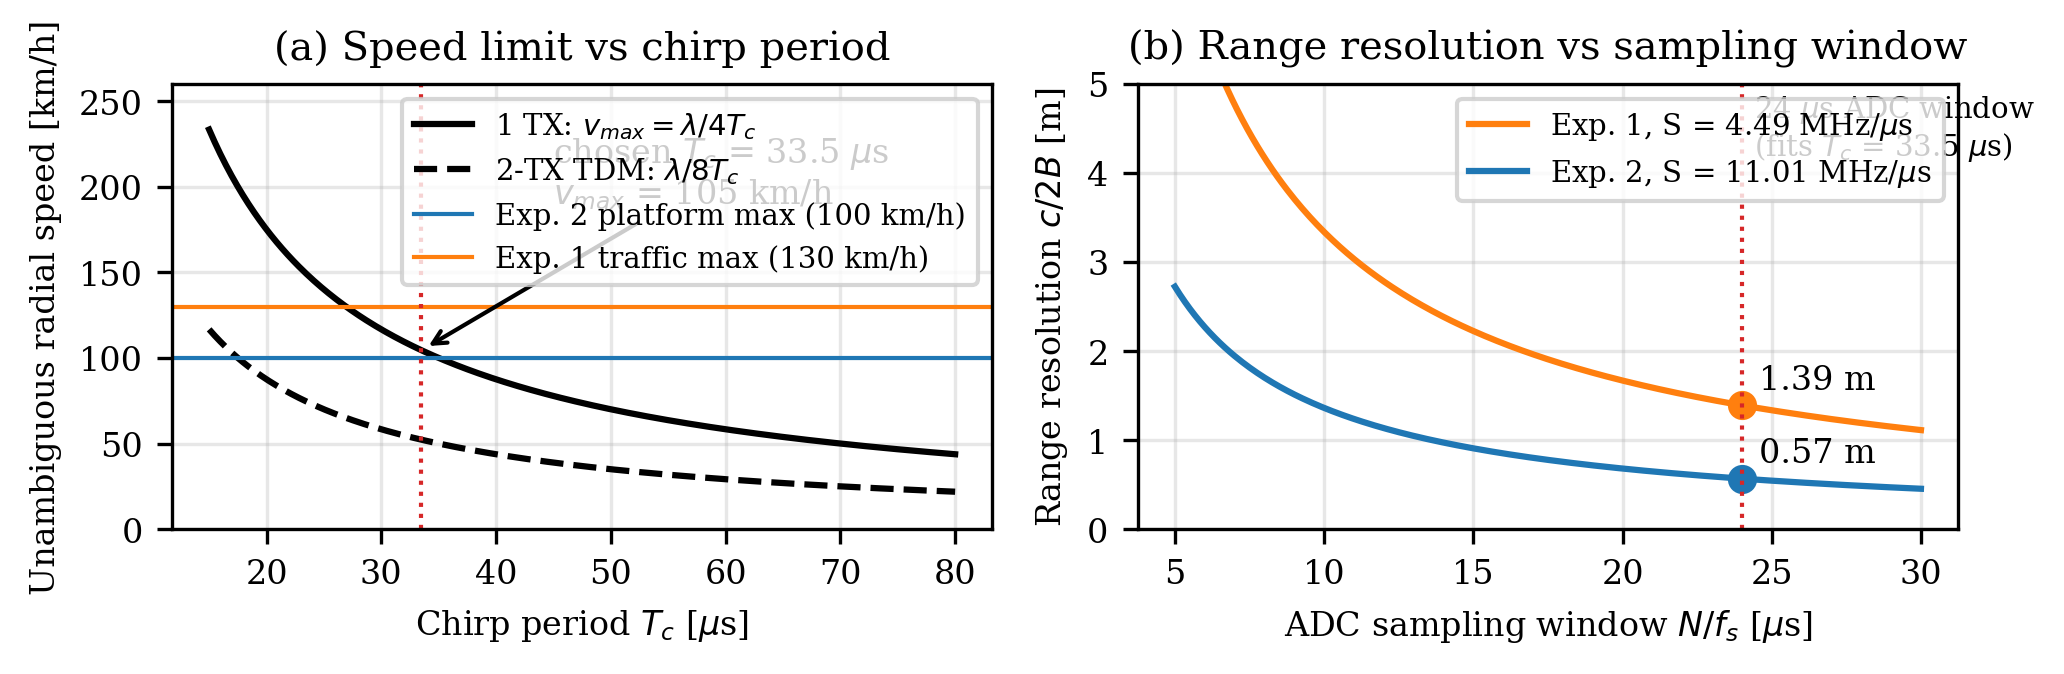
\includegraphics[width=\textwidth]{fig_waveform_design.png}
\caption{Waveform trade-offs. (a) The unambiguous radial speed falls as $1/T_c$, and a second TDM
transmitter halves it. At $T_c=33.5\,\mu$s a single TX covers 105\,km/h, which keeps the
Exp.~2 clutter ridge unaliased up to 100\,km/h. (b) Range resolution is set by the sampled sweep
$S\,N/f_s$. A 24\,$\mu$s window gives 1.39\,m (Exp.~1) and 0.57\,m (Exp.~2).}
\label{fig:waveform}
\end{figure*}

\textbf{Accepted limitations.} In Exp.~1, cars at 120\,km/h exceed $v_{max}$ in radial speed only
beyond about $\pm60^\circ$ azimuth, and the look sweep stops at $\pm60^\circ$. In Exp.~2,
oncoming traffic (closing speed up to about 55\,m/s) wraps in Doppler. These cars are still
detected but their speed is wrong, and speed unwrapping with staggered PRF is future work. At
$L=16$ the velocity resolution is 3.6\,m/s. Halving it ($L=32$, $D=128$) is possible by using
3-frame training pooling.

\subsection{STAP configuration}
Exp.~1 sweeps 9 looks ($-60^\circ$ to $60^\circ$ in $15^\circ$ steps) with 128 Doppler
hypotheses. It pools training over 9 frames: 128 bins $\times$ 9 = 1152 samples, or 2304 after
forward-backward (FB) averaging, which exceeds $2D=1024$. Exp.~2 sweeps 7 looks ($\pm45^\circ$)
with 32 hypotheses. It pools 3 frames, during which the scene moves about 1 range bin per frame
at 50\,Hz: $128\times3=384$ samples, or 768 with FB, which exceeds $2D=128$. Both experiments
use a 15\,dB training censor, $\kappa=1$ noise-eigenvalue loading, Hann temporal taper, EFA with
$Q=3$, and per-hypothesis range CFAR with $P_{FA}=10^{-3}$.

% ======================================================================
\section{Signal Model and Algorithms}
\subsection{FMCW signal and data cube}
The transmit phase is $\phi(t)=2\pi(f_c t+\tfrac12 S t^2)$. An echo with delay
$\tau=2R/c$, mixed as $s_{tx}\,s_{rx}^{*}$, gives the IF phase
\begin{equation}
\psi(t)=2\pi\left(f_c\tau+S t\tau-\tfrac12 S\tau^2\right),\quad f_b=S\tau+\frac{2v_r}{\lambda},
\end{equation}
where $v_r=\dot R$ is positive when the target recedes. For scatterer $s$, virtual channel $c$
(position $\vect p_c=\vect p_{tx}+\vect p_{rx}$), slow-time index $l$ and fast-time sample $n$:
\begin{equation}
X[c,l,n]=\sum_s \alpha_s\, e^{j2\pi f_{b,s} n/f_s}\, e^{j2\pi\nu_s l T_{slow}}\,
e^{-j2\pi\vect p_c\cdot\vect u_s/\lambda}+n[c,l,n],
\end{equation}
with slow-time frequency $\nu=2v_r/\lambda$ and unit direction $\vect u_s$. The simulator
recomputes the exact path length for every chirp, so range migration and range-Doppler coupling
($f_c/S$ metres per m/s) are included.

\subsection{Conventional processing}
\emph{Range:} per-chirp DC removal, window $w_n$, and an $N_{fft}$-point FFT,
$Y[c,l,k]=\sum_n w_n(X[c,l,n]-\bar X_{c,l})e^{-j2\pi kn/N_{fft}}$, with
$R_k=k\,c f_s/(2SN_{fft})$ on the positive beat band.
\emph{Doppler:} a windowed FFT over $l$ for each channel and range bin, $v_q=\lambda\nu_q/2$,
and a non-coherent map $P[k,q]=\sum_c|Z[c,q,k]|^2$.
\emph{Detection:} CA-CFAR with $N$ training cells. A cell is declared when
$P>\alpha\,\bar P_{train}$, with $\alpha=N(P_{FA}^{-1/N}-1)$, which is exact for exponential
(square-law) noise~\cite{finn1968,richards2014}. Detections are grouped by local maxima of the
CFAR-normalised statistic and then refined parabolically.
\emph{Angle:} the Bartlett spectrum $P(\theta)=|\vect a(\theta)\Hm\vect z|^2$ with
$a_c(\theta)=e^{-j2\pi\vect p_c\cdot\vect u(\theta)/\lambda}$ and $\sin\theta=u_x$.

\subsection{Channel calibration}
A corner reflector at known range and angle $\theta_0$ gives the zero-Doppler response
$\bar x_c$ at its range bin, averaged over loops and frames. The calibration is
\begin{equation}
\tilde c_c=\frac{a_c(\theta_0)}{\bar x_c},\qquad
c_c=\frac{\tilde c_c\,|\tilde c_0|/\tilde c_0}{\frac1C\sum_m|\tilde c_m|},
\end{equation}
which references the phase to channel 0 and sets the mean gain to unity, and it is applied as
$V\leftarrow V\odot\vect c$. Quality checks require the reflector SNR to be at least 20\,dB and
the frame-to-frame phase jitter to be at most $5^\circ$. A second capture at a different angle
verifies the angle sign.

\subsection{Space-time model}
For range bin $r$ the snapshot is $\vect x_r\in\mathbb C^{D}$, with $x_r[lC+c]=V[c,l,r]$ and
$D=CL$. For a single TX the steering vector is separable:
\begin{equation}
\vect s(\theta,\nu)=\vect b(\nu)\otimes\vect a(\theta),\quad b_l=e^{j2\pi\nu lT_{slow}}.
\end{equation}
Stationary clutter from angle $\theta$ has $\nu=-2v_p\sin\theta/\lambda$
(Fig.~\ref{fig:ridge}). Its rank is approximately $r_c\approx C+(L-1)\beta$, with
$\beta=4v_pT_{slow}/\lambda$~\cite{ward1994}. For Exp.~2, $\beta=0.48$, 0.58, 0.77 and 0.96 at 50,
60, 80 and 100\,km/h, which gives $r_c\approx11$--19 of $D=64$. For Exp.~1 ($v_p=0$) clutter
lies only at $\nu=0$, with rank of about $C$.

\begin{figure}[t]
\centering
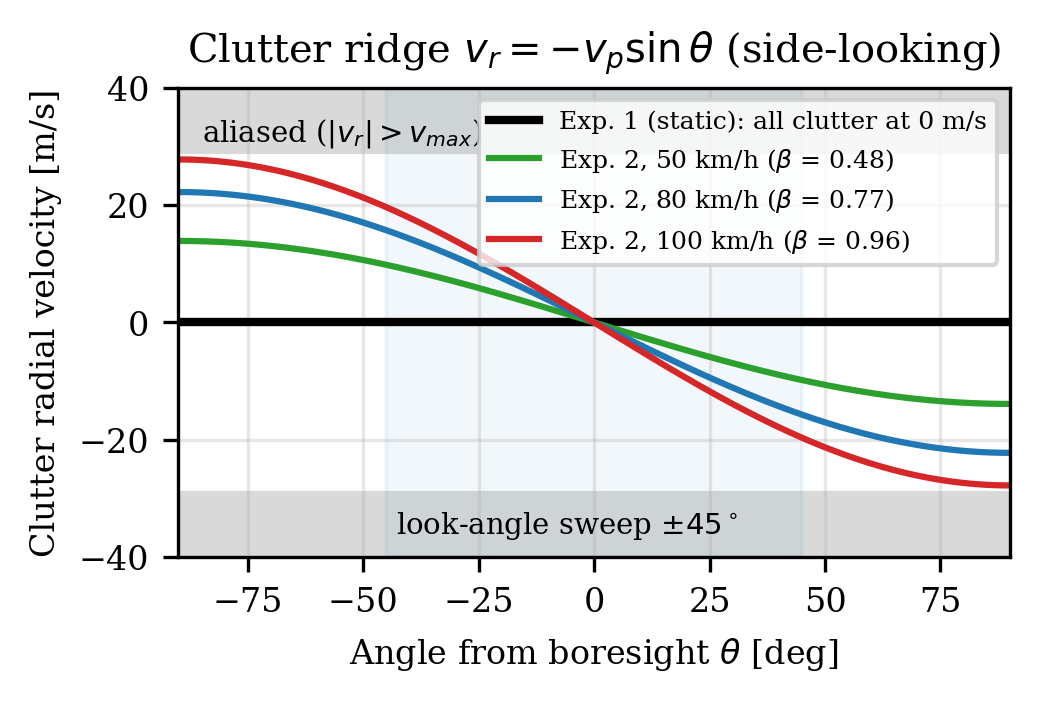
\includegraphics[width=\columnwidth]{fig_clutter_ridge.png}
\caption{Predicted clutter locus. Exp.~1 places all clutter at 0\,m/s. Exp.~2 produces the
side-looking ridge, which stays inside $\pm v_{max}$ ($\beta\le1$) up to 100\,km/h.}
\label{fig:ridge}
\end{figure}

\subsection{Training and covariance estimation}
Training bins for test bin $r$ are the $N_t$ nearest valid bins outside $\pm g$ guard cells. For a
static scene, or a slowly shifting one, they are pooled over $F_t$ consecutive frames centred on
the test frame, giving $K=N_tF_t$ samples. A bin is censored from training if its power exceeds
$10^{\gamma/10}$ times the local median, which prevents strong vehicles from nulling themselves.
The covariance estimate is
\begin{align}
\hat{\vect R}&=\frac1K\sum_{k=1}^{K}\vect x_k\vect x_k\Hm,\qquad
\hat{\vect R}_{FB}=\tfrac12\left(\hat{\vect R}+\vect J\hat{\vect R}^{*}\vect J\right),\\
\hat{\vect R}_\lambda&=\hat{\vect R}_{FB}+\sigma_L\vect I,\quad \sigma_L=\kappa\,\mathrm{mean}\{\text{lowest }25\%\text{ eigenvalues}\}.
\end{align}
FB averaging~\cite{nitzberg1980} is valid for a single-TX uniform linear array with uniform PRI
and calibrated channels, and it doubles the effective $K$. Diagonal loading~\cite{carlson1988}
makes $\hat{\vect R}$ invertible, though it does not make the estimate accurate. The expected
SINR loss of the sample-matrix filter~\cite{rmb1974} is
\begin{equation}
\mathcal L_{RMB}=\frac{K+2-D}{K+1}\quad(\approx-3\text{\,dB at }K=2D).
\end{equation}

\begin{figure}[t]
\centering
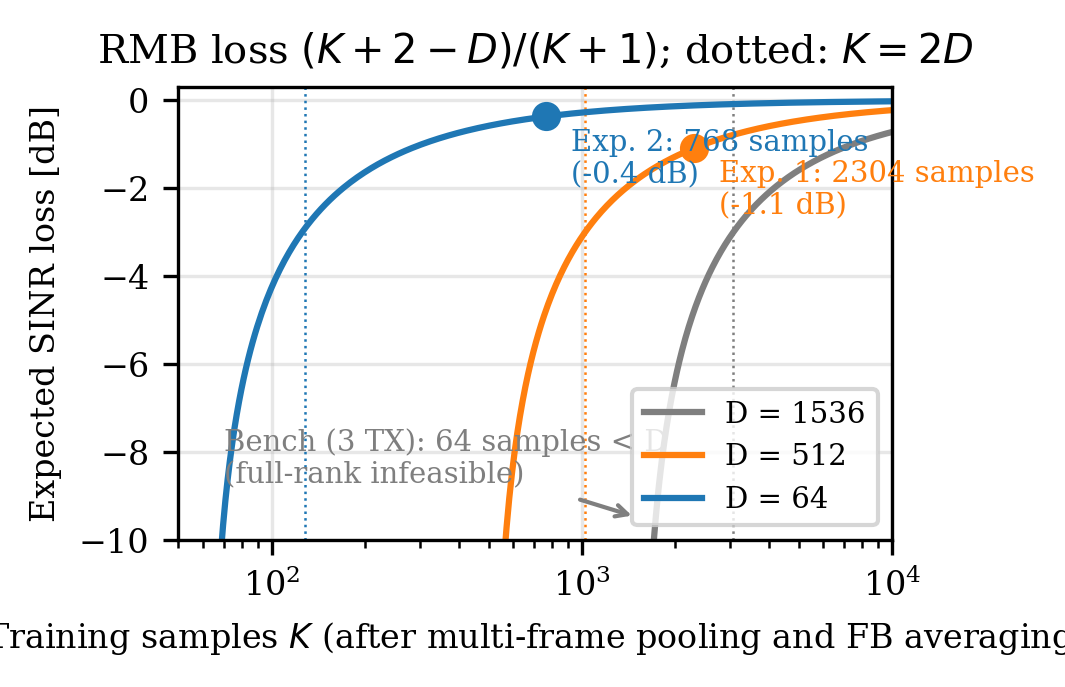
\includegraphics[width=\columnwidth]{fig_sample_support.png}
\caption{Training support against the RMB loss. Multi-frame pooling and FB averaging make
full-rank STAP feasible for both outdoor experiments. The bench waveform was infeasible.}
\label{fig:rmb}
\end{figure}

\subsection{STAP filters}
All filters are distortionless ($\vect w\Hm\vect s=1$) and are evaluated on the same snapshots,
training and hypotheses $\{\vect s_j\}_{j=1}^{J}$, where $J$ = looks $\times$ Doppler
hypotheses.
\begin{itemize}
\item \emph{Non-adaptive:} $\vect w=(\vect t\odot\vect s)/\sum\vect t$, a tapered beamformer
followed by a Doppler filter.
\item \emph{MVDR (full rank):}
$\vect w=\hat{\vect R}_\lambda^{-1}\vect s/(\vect s\Hm\hat{\vect R}_\lambda^{-1}\vect s)$,
computed by Cholesky solve without an explicit inverse.
\item \emph{EFA}~\cite{dipietro1992}: for hypothesis $j$, $\vect T_j=\vect F_j\otimes\vect I_C$,
where $\vect F_j\in\mathbb C^{L\times Q}$ holds $Q$ adjacent tapered Doppler filters. Then
$\tilde{\vect R}_j=\vect T_j\Hm\hat{\vect R}\vect T_j$ is $QC\times QC$ ($=12$),
$\tilde{\vect s}_j=\vect T_j\Hm\vect s_j$, and $\vect w_j=\vect T_j\tilde{\vect R}_j^{-1}\tilde{\vect s}_j/(\cdot)$.
\item \emph{PC eigencanceller}~\cite{haimovich1996}: $\hat{\vect R}=\vect U\vect\Lambda\vect U\Hm$,
$k=\#\{\lambda_i>10\hat\sigma^2\}$, and
$\vect w\propto(\vect I-\vect U_k\vect U_k\Hm)\vect s$.
\item \emph{DPCA}~\cite{ward1994}: the difference
$x_{l+\ell,\text{rear}}-x_{l,\text{front}}$ cancels clutter when
$v_p=d/(2\ell T_{slow})$, which is 29.1\,m/s for $\ell=1$ and 14.5\,m/s for $\ell=2$ in Exp.~2.
\end{itemize}
The output $y_r(j)=\vect w_j\Hm\vect x_r$ is tested with 1-D CA-CFAR along range for each
hypothesis. Detections from neighbouring looks are merged by keeping the strongest look in each
(range, velocity) cell. Performance is scored as output SINR
$|\vect w\Hm\vect g|^2/(\vect w\Hm\vect R_i\vect w)$ against the clairvoyant optimum
$\vect g\Hm\vect R_i^{-1}\vect g$, $P_D$/$P_{FA}$ with Wilson intervals, run time and peak
memory.

\subsection{Computational cost}\label{sec:cost}
The cost per test bin is $\mathcal O(KD^2+D^3/3+JD^2)$ for MVDR, $\mathcal O(KD^2+D^3)$ for PC
and $\mathcal O(J(QC)^3)$ for EFA. Fig.~\ref{fig:cost} shows measured times at the Exp.~1 sizes
($D=512$, $J=9\times128$, $K=1152$). Extrapolated over 153 test bins and 12 frames, MVDR alone
takes about 1\,h on a 4-core CPU. The time is spent inside compiled LAPACK routines, not Python.
The dominant MVDR term is an eigen-decomposition that is used only to set the loading level and
compute diagnostics. This analysis directly motivates Section~\ref{sec:opt}.

\begin{figure*}[t]
\centering
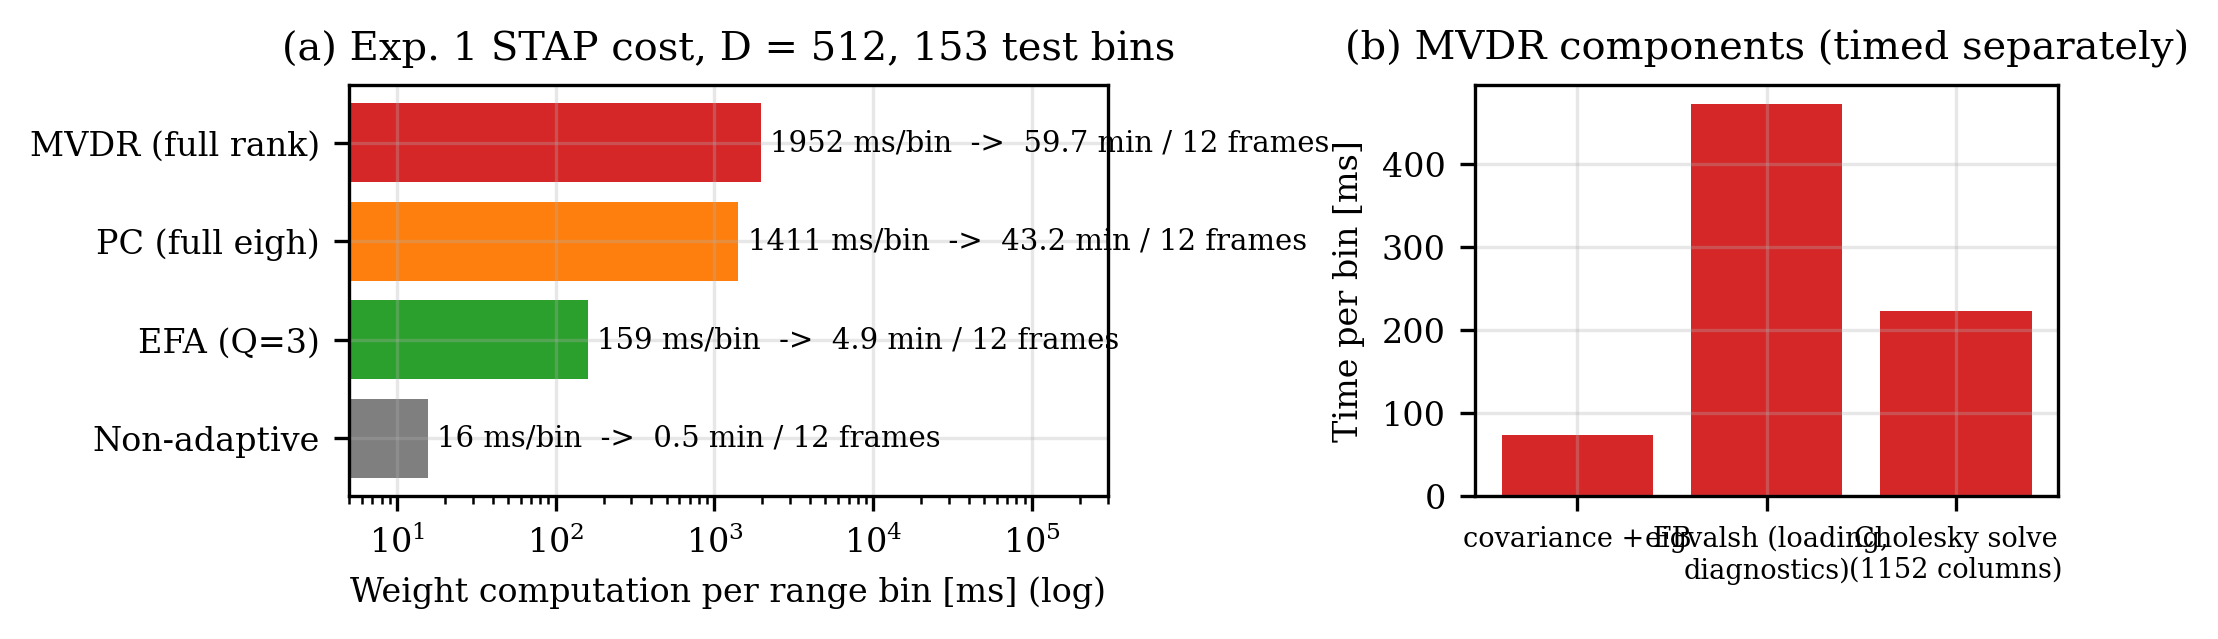
\includegraphics[width=\textwidth]{fig_stap_compute.png}
\caption{Measured STAP weight cost at Exp.~1 sizes (Databricks serverless, 4 vCPU, NumPy/OpenBLAS,
complex128). Timings on a shared machine vary by about $\pm30\,\%$. (a) Per range bin, with the
projection to 153 bins $\times$ 12 frames. (b) MVDR components timed separately: the full
eigen-decomposition dominates.}
\label{fig:cost}
\end{figure*}

% ======================================================================
\section{Data Collection Procedure}
\subsection{Calibration capture (before each experiment)}
\begin{enumerate}
\item Load the experiment waveform; the calibration is waveform-specific.
\item Place a corner reflector at least 8\,m away at boresight, at a height of about 1\,m, in an
open area. At 10\,m the beat frequency is 0.30\,MHz, above the 175\,kHz HPF.
\item Record at least 8 static frames, then run \texttt{scripts/calibrate\_capture.py}. Accept
the result if the reflector SNR is at least 20\,dB and the phase jitter is at most $5^\circ$.
\item Move the reflector to about $+27^\circ$, re-record, and confirm that the angle reported
with the calibration matches. This also confirms the angle sign.
\item Write the result to \texttt{rx\_calibration} in the YAML file. If the radar will operate
behind a radome, calibrate with the radome fitted.
\end{enumerate}

\subsection{Experiment 1: static highway overlook}
The radar is mounted on a 17th-floor balcony (about 51\,m high) overlooking Highway 401. The
slant range to traffic is about 71--226\,m, the depression angle is $13$--$45^\circ$, and
traffic moves at 100--130\,km/h in both directions.
\begin{enumerate}
\item Mount the board on a rigid tripod with the array axis (RX1$\rightarrow$RX4) parallel to the
road and boresight perpendicular to it. Tilt it down by $25$--$30^\circ$. Open the window, because
(low-E) glass can attenuate 77\,GHz by 10--40\,dB.
\item Configure mmWave Studio as in Table~\ref{tab:waveform}: TX1 only, 128 loops, 50\,ms frames,
600 frames (30\,s, 295\,MB), RX gain 30\,dB, LVDS 2-lane DDR.
\item Record several 30\,s captures with photographs and notes on the geometry. Measure the true
height and lane distances and update \texttt{range\_min\_m}/\texttt{range\_max\_m}.
\item Acceptance checks: 0 out-of-range ADC values in the decode report. The two traffic
directions must show opposite velocity signs, with approaching cars giving $v_r<0$, which
verifies the mixer convention. Cars on the known side must have the correct angle sign. Each car
should persist across about 20 frames. Static returns must stay at 0\,m/s, since any drift
indicates a mount problem.
\end{enumerate}

\subsection{Experiment 2: vehicle-mounted side-looking STAP}
\begin{enumerate}
\item Mount the radar on a rigid roof-rack crossbar about 1.8\,m above the road, never on a pole,
because vibration smears the clutter ridge. Use a radar-transparent cover, with the array axis
along the direction of travel and boresight perpendicular to it, tilted down by about $5^\circ$.
Record which end of the array faces forward, because it sets the sign of $\vect v_p$.
\item Configure 16 loops, 20\,ms frames and 3000 frames (60\,s, 184\,MB). Log GPS speed at 1--10\,Hz
with time-aligned timestamps.
\item Drive constant-speed runs at 50, 60, 80 and 100\,km/h on cruise control. Add one run at
52\,km/h, the DPCA matched speed for $\ell=2$. Note traffic in the adjacent lanes.
\item Acceptance checks: the clutter ridge slope must match $-v_p\sin\theta$ from GPS speed
(Fig.~\ref{fig:ridge}), there must be no ridge wrap below 105\,km/h, and the eigenspectrum rank
should be close to the $r_c$ predicted by Brennan's rule.
\item Safety: the driver does not operate the laptop, and a passenger runs the capture.
\end{enumerate}

% ======================================================================
\section{STAP Optimisation Directions}\label{sec:opt}
The goal is lower run time and lower training requirement at a small, quantified SINR or $P_D$
cost. Every candidate is implemented behind the same
\texttt{weights(training, S, nu)} interface and compared with full-rank MVDR on identical data.

\subsection{Implementation speed-ups (no or negligible performance change)}
\begin{itemize}
\item \emph{Remove redundant eigen-decompositions:} take the loading level from a per-frame noise
estimate or the trace, and run diagnostics on a subset of bins. This eigen-decomposition is the
largest of the three timed MVDR components (472 of 769\,ms, Fig.~\ref{fig:cost}b).
\item \emph{Covariance reuse:} neighbouring test bins share almost all of their training. Sliding
rank-one Cholesky updates and downdates cost $\mathcal O(D^2)$ per sample instead of
$\mathcal O(D^3)$ per bin, and sharing one $\hat{\vect R}$ across blocks of about 8 bins gives
about $8\times$.
\item \emph{Structure:} a unitary transform maps a persymmetric Hermitian matrix to a real
symmetric one, so the arithmetic becomes real-valued. For the static scene, a
Toeplitz-block-Toeplitz model allows fast solvers.
\item \emph{Partial eigensolvers} (Lanczos) for PC, since only $k\ll D$ components are needed.
\item \emph{Hardware:} batched solves across bins on a GPU (RTX~3060) in complex64. The consumer
GPU's FP64 throughput is very low, so single precision, stabilised by loading, is required, and
its accuracy must be checked against complex128.
\end{itemize}

\subsection{Reduced-dimension and reduced-rank STAP}
EFA (implemented) and PC (implemented) are the reference points. Further candidates are joint
domain localised (JDL) processing in angle-Doppler beamspace~\cite{wang1994}, pre-Doppler
beamspace filters, and the multistage Wiener filter~\cite{goldstein1998}, which approximates MVDR
in $r\ll D$ stages without an eigen-decomposition. The key trade-off is the reduced dimension $r$
against SINR loss, together with a training requirement of about $2r$ instead of $2D$.

\subsection{Sample-efficient covariance estimation}
Candidates are shrinkage estimators~\cite{ledoit2004} and knowledge-aided STAP
\cite{guerci2006}. In knowledge-aided STAP, a clutter-covariance prior is computed from the
geometry: GPS speed gives $v_p$, the predicted ridge gives $\nu(\theta)$, and the prior is blended
with the sample estimate. Sparse-recovery STAP is a further candidate, in which clutter is
represented on an angle-Doppler dictionary. These methods reduce the dependence on homogeneous
training, which is the main real-world failure mode for road scenes with discretes and lane
edges.

\subsection{Machine-learning directions}
\begin{itemize}
\item \emph{Learned dimension reduction:} learn $\vect T\in\mathbb C^{D\times r}$ (or a
generator for it) offline from simulated clutter. The objective is the output SINR of the
reduced MVDR rather than reconstruction error. The direct baselines are EFA, JDL and PC at
equal $r$. This is the proposed primary research contribution.
\item \emph{Learned covariance and loading:} a small network predicts the loading level,
shrinkage factor or clutter rank from eigenspectrum and power features. This replaces the
heuristics in Section~IV-E.
\item \emph{Deep unfolding}~\cite{monga2021}: unroll a fixed number of conjugate-gradient or MSWF
iterations with learned step sizes, giving a bounded and predictable cost per bin.
\item \emph{Training-sample selection:} a classifier for homogeneous training bins, as an
alternative to power censoring.
\item \emph{End-to-end detection} on angle-Doppler maps (CNN). This is lowest priority, because it
loses the CFAR guarantee and interpretability.
\end{itemize}
The simulator supplies unlimited labelled data. Exps.~1 and~2 measure the gap between simulated
and real data, so a learned method only counts as an improvement if it holds on the real
captures.

% ======================================================================
\section{Plan and Milestones}
\begin{table}[h]
\centering
\caption{Remaining work (ordered).}
\label{tab:plan}
\setlength{\tabcolsep}{3pt}
\begin{tabular}{p{0.3\columnwidth}p{0.62\columnwidth}}
\toprule
Milestone & Deliverable / success criterion\\
\midrule
M1 Exact speed-ups & Exp.~1 STAP at least $10\times$ faster, outputs identical to $10^{-6}$\\
M2 Calibration + Exp.~1 & Verified mixer sign, angle sign, calibration; car tracks across frames\\
M3 Vehicle rig + GPS & Rigid mount, synchronised GPS, timestamp ingestion\\
M4 Exp.~2 captures & 50--100\,km/h runs; ridge matches $-v_p\sin\theta$\\
M5 STAP benchmark & NA / MVDR / EFA / PC / DPCA: $P_D$, false alarms, SINR loss, runtime on real data\\
M6 Optimisation study & JDL/MSWF + learned $\vect T$ against EFA/PC at equal $r$; GPU complex64\\
M7 Final report & Results, limitations, recommendations\\
\bottomrule
\end{tabular}
\end{table}

\textbf{Risks.} The main risks are lower outdoor SNR than the assumed link budget (mitigation:
RX gain up to 36--40\,dB and shorter ranges), mount vibration (rigid crossbar), and
heterogeneous road clutter (censoring and knowledge-aided priors). Speed wrapping of oncoming
traffic is accepted for now and handled later with staggered PRF.

% ======================================================================
\begin{thebibliography}{99}
\bibitem{brennan1973} L.~E. Brennan and I.~S. Reed, ``Theory of adaptive radar,'' \emph{IEEE Trans. Aerosp. Electron. Syst.}, vol.~AES-9, no.~2, pp.~237--252, 1973.
\bibitem{rmb1974} I.~S. Reed, J.~D. Mallett, and L.~E. Brennan, ``Rapid convergence rate in adaptive arrays,'' \emph{IEEE Trans. Aerosp. Electron. Syst.}, vol.~AES-10, no.~6, pp.~853--863, 1974.
\bibitem{ward1994} J.~Ward, ``Space-time adaptive processing for airborne radar,'' MIT Lincoln Laboratory, Tech. Rep. 1015, 1994.
\bibitem{klemm2006} R.~Klemm, \emph{Principles of Space-Time Adaptive Processing}, 3rd~ed. London, U.K.: IET, 2006.
\bibitem{finn1968} H.~M. Finn and R.~S. Johnson, ``Adaptive detection mode with threshold control as a function of spatially sampled clutter-level estimates,'' \emph{RCA Rev.}, vol.~29, pp.~414--464, 1968.
\bibitem{richards2014} M.~A. Richards, \emph{Fundamentals of Radar Signal Processing}, 2nd~ed. New York, NY, USA: McGraw-Hill, 2014.
\bibitem{nitzberg1980} R.~Nitzberg, ``Application of maximum likelihood estimation of persymmetric covariance matrices to adaptive processing,'' \emph{IEEE Trans. Aerosp. Electron. Syst.}, vol.~AES-16, no.~1, pp.~124--127, 1980.
\bibitem{carlson1988} B.~D. Carlson, ``Covariance matrix estimation errors and diagonal loading in adaptive arrays,'' \emph{IEEE Trans. Aerosp. Electron. Syst.}, vol.~24, no.~4, pp.~397--401, 1988.
\bibitem{dipietro1992} R.~C. DiPietro, ``Extended factored space-time processing for airborne radar systems,'' in \emph{Proc. 26th Asilomar Conf. Signals, Syst. Comput.}, 1992, pp.~425--430.
\bibitem{haimovich1996} A.~M. Haimovich, ``The eigencanceler: Adaptive radar by eigenanalysis methods,'' \emph{IEEE Trans. Aerosp. Electron. Syst.}, vol.~32, no.~2, pp.~532--542, 1996.
\bibitem{wang1994} H.~Wang and L.~Cai, ``On adaptive spatial-temporal processing for airborne surveillance radar systems,'' \emph{IEEE Trans. Aerosp. Electron. Syst.}, vol.~30, no.~3, pp.~660--670, 1994.
\bibitem{goldstein1998} J.~S. Goldstein, I.~S. Reed, and L.~L. Scharf, ``A multistage representation of the Wiener filter based on orthogonal projections,'' \emph{IEEE Trans. Inf. Theory}, vol.~44, no.~7, pp.~2943--2959, 1998.
\bibitem{ledoit2004} O.~Ledoit and M.~Wolf, ``A well-conditioned estimator for large-dimensional covariance matrices,'' \emph{J. Multivariate Anal.}, vol.~88, no.~2, pp.~365--411, 2004.
\bibitem{guerci2006} J.~R. Guerci and E.~J. Baranoski, ``Knowledge-aided adaptive radar at DARPA,'' \emph{IEEE Signal Process. Mag.}, vol.~23, no.~1, pp.~41--50, 2006.
\bibitem{monga2021} V.~Monga, Y.~Li, and Y.~C. Eldar, ``Algorithm unrolling: Interpretable, efficient deep learning for signal and image processing,'' \emph{IEEE Signal Process. Mag.}, vol.~38, no.~2, pp.~18--44, 2021.
\end{thebibliography}

\end{document}
